% !TEX root = ./Vorlesungsmitschrift AGLA 2.tex  
\lecture{Fr 26.06. 10:15}{}
\file{Projektive Quadriken Teil 1}
\section{Quadriken}\label{projektive_quadriken}
Sei \( K \) ein Körper und \( Z\subseteq \projectionspaceover{n}{K} \) ein projektiver Unterraum. Dann ist \( Z=\projectionspace{W} \) für \(Z\subseteq \projectionspaceover{n}{K} \) ein projektiver Unterraum. Dann ist \( Z=\projectionspace{W} \) für \( W\untervektorraum K^{n+1} \) ein \( K \)-Untervektorraum. Sei \( W \) gegeben durch
\begin{equation*}
  W=\Set{(x_0,\dotsc,x_n)\in K^{n+1}|a_{i0}x_0+\dotsb+a_{in}x_n=0,\quad 1\leq i\leq r}
\end{equation*}
für Koeffizienten \( a_{ij}\in K  \), \( 1\leq i \leq r \), \( 0\leq j\leq n \). Wir können \( Z \) auffassen als
\begin{equation*}
  Z=\set{(\braceannotate{\in Z}{(x_0:\dotsc:x_n)})\in \projectionspaceover{n}{K}\maps a_{i0}x_0+\dotsb+a_{in}x_n=0\quad 1\leq i\leq r}.
\end{equation*}
\begin{frage*}
  Was passiert, wenn wir die \emph{linearen} Formen \( a_{i0}x-0+\dotsb+a_{in}x_n \) durch allgemeine Polynome in \( x_0,\dotsc,x_n \) ersetzen.
\end{frage*}
\emph{In diesem Abschnitt:} \( r=1 \) und wir ersetzen die Linearform \( a_{10}x_0+\dotsb+a_{1n}x_n=0 \) durch ein \emph{quadratisches Polynom}.
\begin{definition*}
  Sei \( K \) ein Körper. Wir nenne einen Ausdruck der Form
  \begin{equation*}
    P(x_0,\dotsc,x_n)=\sum_{\mathclap{0\leq i\leq j\leq n}}\alpha_{ij}x_i x_j
  \end{equation*}
  mit \( \alpha_{ij}\in K \), \( 0\leq i\leq j\leq n \) ein homogenes Polynom zweiten Grades / eine quadratische Form in den Unbestimmten \( x_0,\dotsc,x_n \).
\end{definition*}
\begin{beispiel*}
  \( x_0^2+x_1^2-x_2^2 \) ist ein homogenes Polynom zweiten Grades, aber \( x_0^2+_1^2+2x_2 \)  nicht.
\end{beispiel*}
\begin{bemerkungen*}
  \begin{enumerate}
    \item Quadratische Formen in den Unbestimmten \( x_0,\dotsc,x_n \) können parametisiert werden durch Tupel
    \begin{equation*}
      \p*{\alpha_{ij}}_{0\leq i\leq j\leq n}\in K^{\binom{n+2}{2}},
    \end{equation*}
    also durch \( \frac{1}{2}(n+2)8(n+1) \) Koeffizienten.
    \item Jedes Polynom \( P(x_0,\dotsc,x_n)\in \polynomials{K}{x_0,\dotsc,x_n} \) induziert eine Abbildung
    \begin{align}
      K^{n+1}&\to K\\
      K^{n+1}\ni(t_0,\dotsc,t_n) &\mapsto P(t_0,\dots,t_n)=\sum_{\mathclap{0\leq i\leq j\leq n}}\alpha_{ij}t_i t_j\in K
    \end{align}
    Sei \( P(x_0,\dotsc,x_n) \) eine quadratische Form und betrachte die Nullstellenmenge
    \begin{equation*}
      X=\Set{(x_0,\dotsc,_n)\in K^{n+1}|P(x_0,\dotsc,x_n)=0}.
    \end{equation*}
    Für \( (x_0,\dotsc,x_n)\in X\Minuszero \) ist dann die gesamte Gerade \( K\cdot(x_0,\dotsc,x_n) \) in \( X \) enthalten, denn für \( \lambda\in K \) ist 
    \begin{equation*}
      P(\lambda x_0,\dotsc,\lambda x_n)=\lambda^2 \braceannotate{=0}{P(x_0,\dotsc,x_n)}=0
    \end{equation*}
  \end{enumerate}
\end{bemerkungen*}
\begin{definition*}
  Wir nennen eine Teilmenge \( C\subseteq K^{n+1} \) ein Kegel falls für jedes \( (x_,\dotsc,x_n)\in C \) und \( \lambda\in K \) gilt
  \begin{equation*}
    (\lambda x_0,\dotsc,\lambda x_n)\in C.
  \end{equation*}
\end{definition*}
\begin{bemerkung*}
  Jeder Kegel \( C\neq \emptyset \) enthält \( (0,\dotsc,0) \).
\end{bemerkung*}
\begin{beispiel}
  Sei \( P=x_0^2+x_1^2-x_2^2 \) und
  \begin{equation*}
    C=\Set{(x_0,x_1,x_2)\in K^3|P(x_0,x_1,x_2)=0}.
  \end{equation*}
  Dann ist \( C \) ein Kegel.
  \begin{figure}[H]
    \centering
    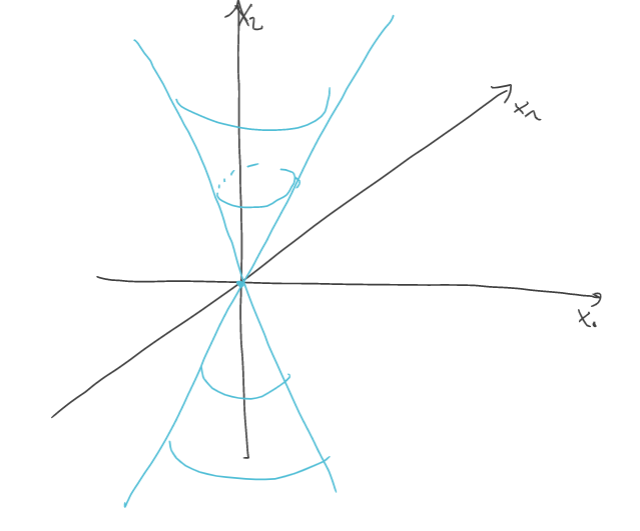
\includegraphics[width=0.8\linewidth]{kreiskegel}
    \label{fig:kreiskegel}
  \end{figure}
  
\end{beispiel}
\begin{beispiel}
  Sei \( Y\subseteq K^2 \) und
  \begin{equation*}
    X\definedas\Set{(ty_1,ty_2,t)\in K^3| t\in K,\logicspace (y_1,y_2)\in Y}.
  \end{equation*}
  Dann ist \( X\subseteq K^3 \).
  \begin{figure}[H]
    \centering
    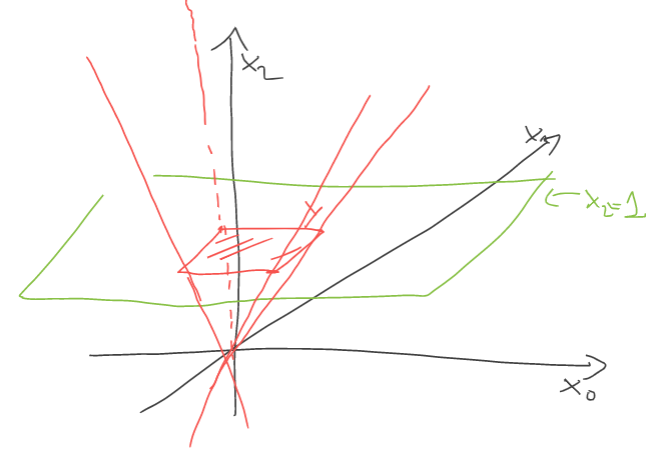
\includegraphics[width=0.8\linewidth]{mengenkegel}
    \label{fig:mengenkegel}
  \end{figure} 
\end{beispiel}
Sei \( C\subseteq K^{n+1} \) ein Kegel. Dann definieren wir
\begin{equation*}
  \projectioncone{C}\definedas \Set{K\cdot v\in \projectionspaceover{n}{K}|K\cdot \subseteq C}.
\end{equation*}
\begin{definition*}
  Sei \( P(x_0,\dotsc,x_n) \) ein homogenes Polynom zweiten Grades mit Koeffizienten in einem Körper \( K \),
  \begin{equation*}
    C\definedas \Set{(x_0,\dotsc,x_n)\in K^{n+1}|P(x_0,\dotsc,x_n)=0}.
  \end{equation*}
  Dann nennen wir \( Q\definedas \projectioncone{C} \) eine (projektive) Quadrik.
\end{definition*}
\begin{bemerkung*}
  Ist \( P(x_0,\dotsc,x_n) \) eine quadratische Form, dann schreiben wir auch
  \begin{equation*}
    Q=\Set{(x_0:\dotsc:x_n)\in \projectionspaceover{n}{K}|P(x_0,\dotsc,x_n)=0}.
  \end{equation*}
\end{bemerkung*}
\begin{konvention*}
  Sei für den Rest des Abschnitts \ref{projektive_quadriken} \( K \) ein Körper mit \( \characteristic{K}\neq 2 \).
\end{konvention*}
\subsection*{Matrixdarstellung von projektiven Quadriken}
\begin{beispiel*}
  Betrachte die projektive Quadrik
  \begin{equation*}
    Q=\Set{(x_0:x_1:x_2)\in \projectionspaceover{2}{K}|x_0^2+x_1^2=x_2^2}
  \end{equation*}
  Dann können wir \( Q \) auch schreiben als \( Q=\projectioncone{C} \) mit
  \begin{equation*}
    C=\Set{(x_0,x_1,x_2)\in K^3|x_0^2+x_1^2-x_2^2=\begin{pNiceMatrix} x_0 & x_1 &x_2 \end{pNiceMatrix}\begin{pNiceMatrix} 1 & 0 & 0 \\ 0 & 1 & 0 \\ 0 & 0 & -1 \end{pNiceMatrix}\begin{pNiceMatrix} x_0 \\ x_1 \\ x_2 \end{pNiceMatrix}=0}.
  \end{equation*}
  Im Allgemeinen:
  Sei
  \begin{equation*}
    P(x_0,\dotsc,x_n)=\sum_{\mathclap{0\leq i \leq j\leq n}\alpha_{ij}x_i x_j}
  \end{equation*}
  ein homogenes Polynom zweiten Grades über einem Körper \( K \) (\( \characteristic-{K}\neq 2 \)). Wir definieren eine Matrix
  \begin{equation*}
    A=\p*{\alpha_{ij}}_{0\leq i,j\leq n}\in \sqmatrices{(n+1)}{K}
  \end{equation*}
  durch
  \begin{equation*}
    \alpha_{ij}=\begin{cases}
      \alpha_{ii} & i=j\\
      \frac{1}{2}\alpha_{ij}&i<j\\
      \frac{1}{2}\alpha_{ji}&i>j.
    \end{cases}
  \end{equation*}
  Schreibe \( \underline{x}=(x_0,\dotsc,x_n)\in K^{n+1} \). Dann ist
  \begin{equation*}
    P(x_0,\dotsc,x_n)=\transpose{\underline{x}}A\underline{x}.
  \end{equation*}
  Sei \( Q=\projectioncone{C} \) mit
  \begin{equation*}
    C=\Set{\underline{x}\in K^{n+1}|\transpose{\underline{x}}A\underline{x}=0}
  \end{equation*}
  und
  \begin{equation*}
    Q=\Set{(x_0:\dotsc:x_n)\projectionspaceover{n}{K}|\transpose{\underline{x}}A\underline{x}=0}.
  \end{equation*}
\end{beispiel*}
\begin{bemerkung*}
  \begin{enumerate}
    \item Für \( \lambda\in \fieldwithoutzero{K} \) gilt auch 
    \begin{equation*}
      Q=\Set{(x_0:\dotsc:x_n)\in \projectionspaceover{n}{K}|\transpose{\underline{x}}(\lambda\cdot A)\underline{x}=0}.
    \end{equation*}
    \item Wir können \( A \) als symmetrische Bilinearform \( S \) auffassen, indem wir
    \begin{equation*}
      S(\underline{x},\underline{y})=\transpose{\underline{x}}A\underline{x}
    \end{equation*}
    setzen für \( \underline{x},\underline{y}\in K^{n+1} \).
  \end{enumerate}
\end{bemerkung*}
\begin{lemma}\label{projektivitaet_projektive_quadriken_auf_projektive_quadriken}
  Sei \( K \) ein Körper, \( \characteristic-{K}\neq 2 \), \( f\maps \projectionspaceover{n}{K}\to\projectionspaceover{n}{K} \) eine Projektivität und \( Q\subseteq \projectionspaceover{n}{K} \) eine Quadrik. Dann ist auch \( f(Q)\subseteq \projectionspaceover{n}{K} \) eine Quadrik.
\end{lemma}
\begin{proof}
  Sei \( f=\projectionmap{F} \) für einen Vektorraumisomorphismus \( F\maps K^{n+1}\to K^{n+1} \). Sei \( S\in \invertiblematrices{n+1}{K} \) die Matrix, die \( F \) in der Standardbasis beschreibt, \dh \( F(\underline{x})=S\cdot \underline{x}\quad \forall \underline{x}\in K^{n+1} \). Sei \( A\in \sqmatrices{(n+1)}{K} \) eine symmetrische Matrix, sodass gilt
  \begin{equation*}
    Q=\Set{(x_0,\dotsc,x_n)\in \projectionspaceover{n}{K}|\transpose{\underline{x}}Ax\underline{x}=0}.
  \end{equation*}
  Dann ist \( f(Q)=\projectioncone{F(C)} \) mit
  \begin{align*}
    F(C)&=\Set{F(x_0,\dotsc,x_n)\in K^{n+1}|\transpose{x}A\underline{x}=0}\\
    &=\set{\braceannotate{\mathclap{=\underline{y}\implies \underline{x}=\inverse{S}\underline{y}}}{S\cdot\underline{x}}\in K^{n+1}|\transpose{\underline{x}}A\underline{x}=0}\\
    &=\Set{\underline{y}\in K^{n+1}\transpose{y}\transpose{\inverse{S}}A\inverse{S}\underline{y}=0}.
  \end{align*}
  Die Matrix \( \transpose{\inverse{S}}A\inverse{S} \) ist symmetrisch und es ist
  \begin{equation*}
    f(Q)=\Set{(x_0:\dotsc:x_n)\in \projectionspaceover{n}{K}|P'(\underline{x})=0}
  \end{equation*}
  mit \( P'(\underline{x})=\transpose{\underline{x}}\transpose{\inverse{S}}A\inverse{S}\underline{x} \).
\end{proof}
\begin{ziel*}
  Verwende Koordinatentransformation \( f\maps \projectionspaceover{n}{K}\to\projectionspaceover{n}{K} \) wie in \thref{projektivitaet_projektive_quadriken_auf_projektive_quadriken} um eine projektive Quadrik \( Q \) in \enquote{möglichst einfacher Form} zu beschreiben.
\end{ziel*}
Ist \( Q=\Set{(x_0,\dotsc,x_n)\in \projectionspaceover{n}{K}|\transpose{\underline{x}}A\underline{x}=0} \) für eine symmetrische Matrix \( A\in \sqmatrices{(n+1)}{K} \), so suchen wir eine Transformationsmatrix \( T\in \invertiblematrices{n+1}{K} \), sodass
\begin{equation*}
  \transpose{T}AT
\end{equation*}
möglichst einfache Gestalt hat.
\begin{bemerkung*}
  Für \( K=\reals \) entspricht dies einem Basiswechsel für die symmetrische Bilinearform \( s(\underline{x},\underline{y})\definedas \transpose{\underline{x}}A\underline{y} \).
\end{bemerkung*}
\file{Projektive Quadriken Teil 2}
\subsection*{Hauptachsenform}
\begin{satz}\label{projektive_quadriken_hauptachsenform}
  Sei \( Q\subseteq \projectionspaceover{n}{\reals} \) eine Quadrik. Dann gibt es eine Koordinatentransformation
  \begin{equation*}
    f\maps \projectionspaceover{n}{\reals}\to\projectionspaceover{n}{\reals}
  \end{equation*}
  und ganze Zahlen \( -1\leq k\leq m\leq n \), sodass
  \begin{equation*}
    f(Q)=\Set{(x_0:\dotsc:x_n)\in \projectionspaceover{n}{\reals}|x_0^2+\dotsb+x_k^2-x_{k+1}^2-\dotsb-x_m^2=0}.
  \end{equation*}
  Zu einer Quadrik \( Q\subset \projectionspaceover{n}{\complexs} \) gibt es eine Koordinatentransformation \( g\maps \projectionspaceover{n}{\complexs}\to \projectionspaceover{n}{\complexs} \) und eine ganze Zahl \( -1\leq m\leq n \) mit
  \begin{equation*}
    g(Q)=\Set{(x_0:\dotsc:x_n)\in \projectionspaceover{n}{\complexs}|x_0^2+\dotsb+x_m^2=0}
  \end{equation*}
  
\end{satz}
\begin{bemerkung*}
  Im Fall \( K=\reals \) kann man \thref{projektive_quadriken_hauptachsenform} aus der Hauptachsenform für symmetrische reelle Matrizen ableiten. Allgemeiner zeigen wir folgendes Resultat:
\end{bemerkung*}
\begin{lemma}\label{symmetrische_bilinearform_diagonalisierung}
  Sei \( K \) ein Körper mit \( \characteristic-{K}\neq 2 \), \( V \) ein \( K \)-Vektorraum der Dimension \( n \) und \( s\maps V\times V\to K \) eine symmetrische Bilinearform. Dann existiert eine Basis \( v_1,\dotsc,v_n\in V \) mit 
  \begin{equation*}
    s(v_i,v_j)=0\quad i\neq j.
  \end{equation*}
\end{lemma}
\begin{proof}
  Induktion nach \( \dim-{V}=n \).
  \begin{proofdescription}
    \item[\( n=0, n=1 \)] \checkmark.
    \item[\( n\geq 2 \)] \begin{enumerate}[label=Fall \rechtsklammer{\alph*}]
      \item \( s(v,v)=0 \) für alle \( v\in V \). Für beliebige \( v_1,v_2\in V \) berechnen wir
      \begin{equation*}
        s(v_1,v_2)=\frac{1}{2}(\braceannotate{=0}{s(v_1+v_2,v_1+v_2)}-\braceannotate{=0}{s(v_1,v_0)}-\braceannotate{=0}{s(v_2,v_2)})=0.
      \end{equation*}
      Wähle nun eine beliebige Basis für \( V \).
      \item Es existiert eine Vektor \( v_1\in V \) mit \( s(v_1,v_1)\neq 0 \). Sei 
      \begin{equation*}
        W\definedas \Set{w\in V|s(v_1,w)=0}.
      \end{equation*}
      \begin{behauptung}
        Es gilt \( V=K\cdot v_1\oplus W \).
      \end{behauptung}
      \emph{denn:} \begin{itemize}
        \item \( K\cdot v_1\cap W=\zeroset \)
        \item für \( v\in V \) ist \( \tilde{v}=\frac{s(v_1,v)}{s(v_1,v_1)}\cdot v_1\in K\cdot v_1 \) und
        \begin{equation*}
          S(v_1,v-\tilde{v})=s(v_1,v)-s(v_1,v_1)\cdot\frac{s(v_1,v)}{(v_1,v_1)}=0
        \end{equation*}
        also \( v-\tilde{v}\in W \) und \( v\in K\cdot v_1+W \).

        Aus \( V=K v_1\oplus W \) folgt
        \begin{equation*}
          \dim-{W}=n-1.
        \end{equation*}
        Nach Induktionsannahme existiert eine Basis \( v_2,\dotsc,v_n \) von \( W \) mit \( s(v_i,v_j)=0 \) für \( 2\leq i,j\leq n \). Nach Konstruktion von \( W \) gilt auch
        \begin{equation*}
          s(v_i,v_j)=0\quad 1\leq i,j\leq n
        \end{equation*}
        und \( v_1,\dotsc,v_n \) ist Basis von \( V \).
      \end{itemize}
    \end{enumerate} 
  \end{proofdescription}
  
\end{proof}